\documentclass[a4paper,12pt]{article}
\usepackage[a4paper, total={6.5in, 10.5in}]{geometry}
%\usepackage[square,sort,comma]{natbib}
\usepackage[R,stopserver]{runcode}
\setminted[R]{fontsize=\footnotesize,linenos=none, frame=single, bgcolor=bg, breaklines=true,escapeinside=||}
\usepackage{pifont} % ding
%\usepackage{circledsteps}

\newcommand{\dcircle}[1]{\ding{\numexpr181 + #1}}
\newcommand{\func}[1]{\textit{#1}}
\newcommand{\pkg}[1]{\textbf{#1}}

\usepackage{caption}
%\usepackage{subcaption}
\usepackage{subfig}

% Title Page
\title{Automated Model Building and Goodness-of-fit via Quantile Regression}
\author{Haim Bar}

\begin{document}
\maketitle
\abstract{This repository contains code and data used in the paper \textit{Automated Model Building and Goodness-of-fit via Quantile Regression} by Bar, Booth, and Wells. Given $P$ predictors $x_i$ and $n$ observations for each $x_i$ and a response variable $y$, the goal is to build a model, $y=f(x_1,\ldots,x_P)$ where $f()$ consists of combinations of powers of the $x_i$'s, which fits the data well across multiple quantiles.}

\section{Prerequisites}
In order to run the code you must first install the \pkg{QREM} package. Since \pkg{QREM} has a model selection option for cases in which the number of predictors is large you also need to install the packages \pkg{edgefinder} and \pkg{SEMMS}. The recommended way to install these packages is from the GitHub repository:

\begin{Verbatim}
devtools::install_github("haimbar/edgefinder")
devtools::install_github("haimbar/SEMMS")
devtools::install_github("haimbar/QREM")
\end{Verbatim}

The model building algorithm is implemented in a function called \func{fitQRloop} in the file runQREM.R. The function takes five arguments:
\begin{itemize}
 \item \textcolor{blue}{M} the data matrix with $P$ columns and $n$ rows.
 \item \textcolor{blue}{qns} The quantile which will be used in the fitting algorithm.
 \item \textcolor{blue}{minDiff} The minimal improvement in the overall goodness of fit in order to accept a new term.
 \item \textcolor{blue}{maxdeg} The maximum degree of any term in the model.
 \item \textcolor{blue}{maxrows} The maximum number of possible terms up to degree maxdeg.
\end{itemize}
The file initSim.R contains the values we used by default. It also contains three other variables which are used by \pkg{QREM} in the fitting process:
\begin{itemize}
 \item \textcolor{blue}{mxm} The maximum number of segments in the partition of the selected variable.
 \item \textcolor{blue}{alphaQ} The level of the goodness of fit test.
 \item \textcolor{blue}{plotit} A Boolean variable which tells the function \func{flatQQplot} whether to show intermediate diagnostic plots for each accepted new term in the model.
\end{itemize}

\showCode{R}{Code/initSim.R}[3][10]

\section{A Univariate Example}
The file Code/Univariate02.R  contains the code for example \#1 in the paper, where $f(x)=x^{5}e^{-x}$ and the random noise is normally distributed with mean 0 and standard deviation which grows linearly with $x$, $sd=0.25(x+0.05)$.
\showCode{R}{Code/Univariate02.R}[3][15]
\runR{Code/Univariate02.R}{Univariate02}[cache]
\noindent The fitted quantile regression models are shown as red curves in Figure \ref{Example1}.

\begin{figure}[b!]
\centering
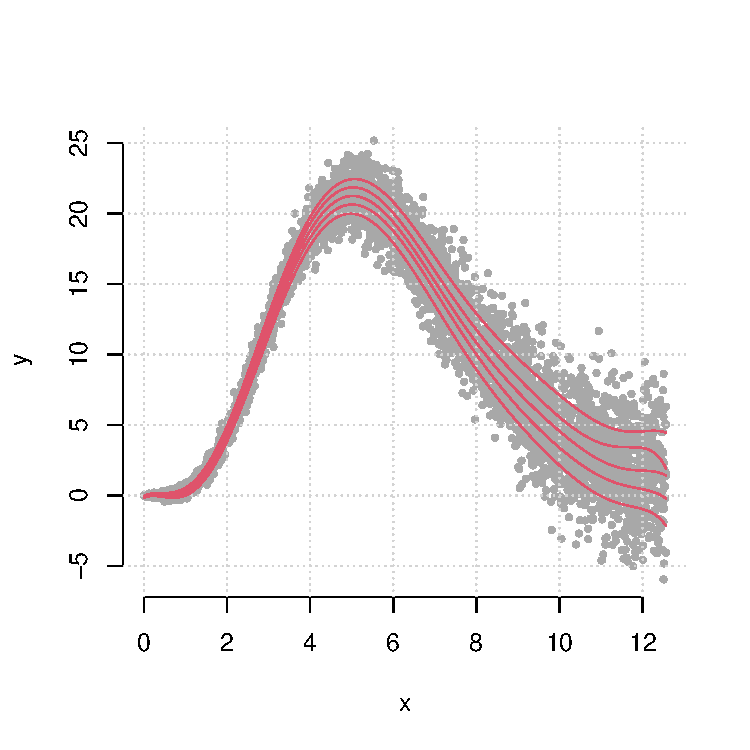
\includegraphics[width=.6\linewidth]{Figures/Uni02.pdf}
\caption{The fitted QR model for $q=1/6,\ldots,5/6$ where the true model is $f(x)=x^{5}e^{-x}$ with random errors i.i.d. $N(0, [0.25(x+0.05)]^2)$.}\label{Example1}
\end{figure} 
 
%\includeOutput{Univariate02}[tex]	


\section{A Multivariate Example}
The program in Code/multivariate04.R generates a data matrix with 2,000 observations and 4 predictors, but only $x_1, x_2, x_4$ are related to the response,
$$y = x_1x_2x_4 + \epsilon$$
and the random errors are i.i.d. $\epsilon\sim N(0, 0.1^2)$

\showCode{R}{Code/multivariate04.R}[1][14]
\runR{Code/multivariate04.R}{multivariate04}%[cache]

The fitted model is: \inlnR{```cat(fittedModel)```}[vbox]
\noindent The predicted values are very close to the observed one, as can be  seen in Figure \ref{multivariate04}.

\begin{figure}[b!]
\centering
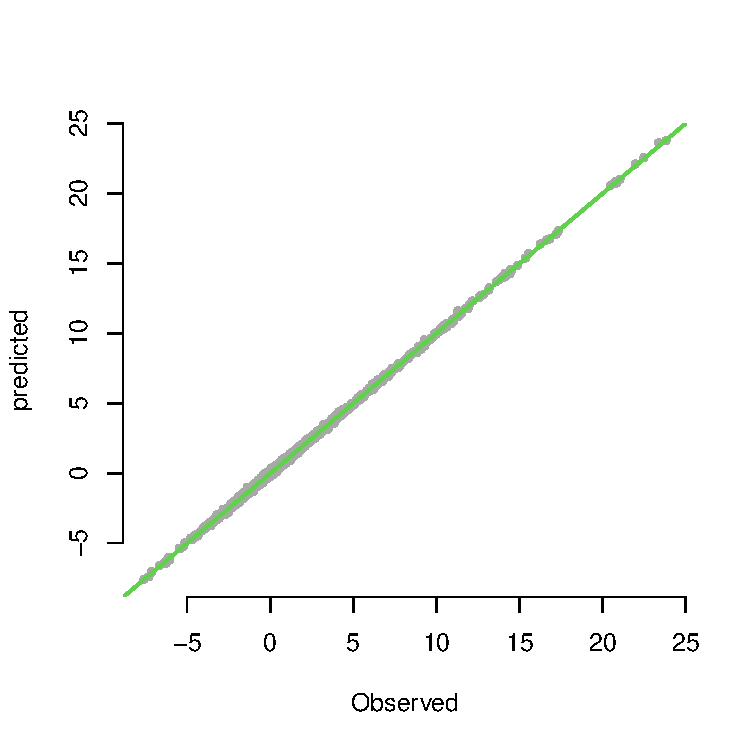
\includegraphics[width=.6\linewidth]{Figures/multivariate04.pdf}
\caption{Fitted QR model vs. observed values for $q=1/2$ where the true model is $f(x_1, x_2, x_3, x_4)=x_1x_2x_4$ with random errors i.i.d. $N(0, 0.1^2)$.}\label{multivariate04}
\end{figure} 

Examples which involve more complicated models with more than one predictor may take a few minutes to run. 

% The file Code/Friedberg7.R contains a multivariate example from the paper XXX, where the data matrix has 20 predictors, but only $x_1-x_5$ are related to the response,
% $$y = 10sin(\pi x_1x_2) + 20(x_3-0.5)^2 + 10x_4 + 5x_5 + \epsilon$$
% and the random errors are i.i.d. $\epsilon\sim N(0, 0.1^2)$
% 
% \showCode{R}{Code/Friedberg7.R}[10][19]
% \runR{Code/Friedberg7.R}{Friedberg7}%[cache]
% 
% Note that this example which involves a more complicated model with five predictors take a few minutes to run. The fitted model is: \inlnR{```cat(fittedModel)```}[vbox]
% \includeOutput{Friedberg7}[vbox]	
% 
% The algorithm did not select any variables which are not related to the response, and the terms in the fitted model represent the true model well. For example, $x_4$ and $x_5$ appear as linear terms in the model, and $x_3$ as quadratic. The combination of powers of $x_1$ and $x_2$ provide a good approximation for the $sin(\pi x_1x_2)$ term in the true model.
% The predicted values are very close to the observed one, as can be  seen in Figure \ref{Friedberg7}
% \showCode{R}{Code/Friedberg7.R}[22][26]
% 
% \begin{figure}[b!]
% \centering
% 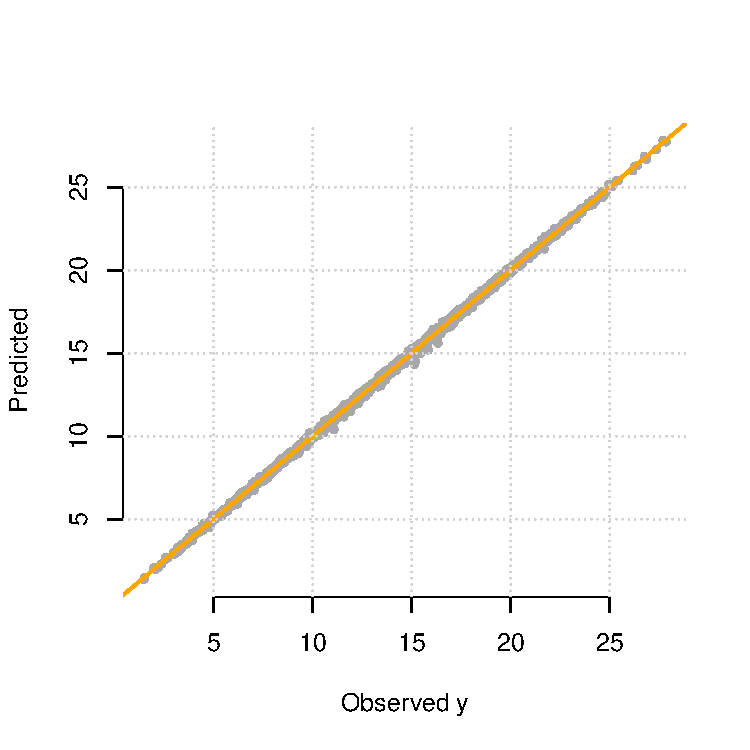
\includegraphics[width=.6\linewidth]{Figures/Friedberg7.pdf}
% \caption{Fitted QR model vs. observed values for $q=1/2$}\label{Friedberg7}
% \end{figure} 

\section{Case Studies}
The repositories contains several case studies:
\begin{itemize}
 \item Concrete.R - predicting the strength of concrete XXX. (Note that fitting a model to this dataset is time-consuming. Saved results can be found in concreteResultsR2s.RData).
 \item mpgreg.R - which factors contribute to gasoline consumption. (We run it 10 times, and it takes a minute or two to finish). The file MPG.py contains a python program which uses TensorFlow to fit the MPG data. The code was obtained from the TensorFlow documentation.
 \item bankNotes.R (a classification example, see https://archive.ics.uci.edu/ml/datasets/banknote+authentication).
 \item Lidar.R - Lidar readings data (univariate, demonstrating data augmentation).
 \item uscrime.R - FBI rape rate data by state (demonstraing regression discontinuity).
 \item Ozone.R - Ozone data.
\end{itemize}

In this section we use the MPG data
\runR{Code/mpgreg.R}{mpg}%[cache]

The fitted model is: \inlnR{```print(summCoef, digits = 3)```}[vbox]
\noindent The predicted values are plotted versus the observed one in Figure \ref{mpgplot}.

\begin{figure}[b!]
\centering
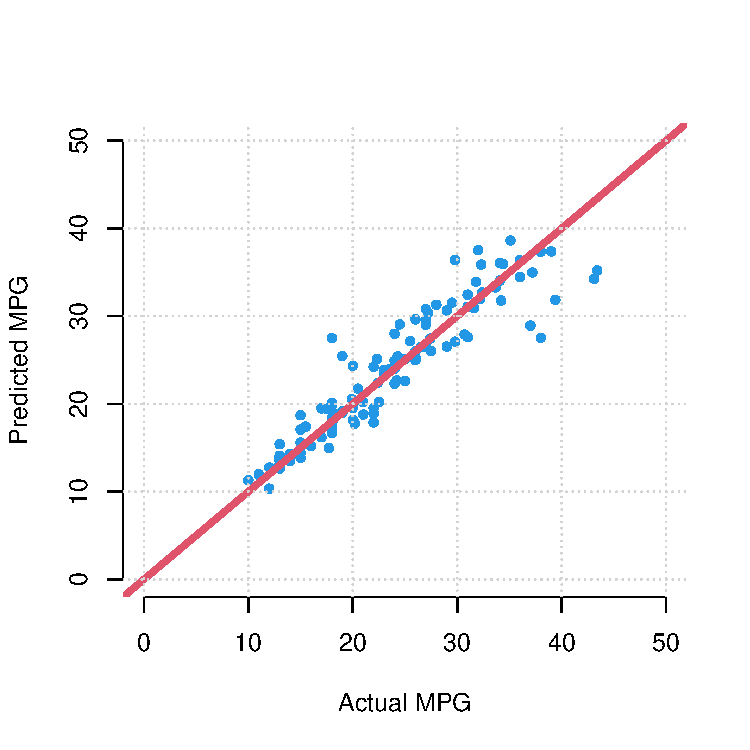
\includegraphics[width=.6\linewidth]{Figures/mpg.pdf}
\caption{Fitted QR model vs. observed values for $q=1/2$ for the MPG data.}\label{mpgplot}
\end{figure} 


% In this section we use the ozone data 
% 
% \runR{Code/Ozone.R}{O3}%[cache]
% 
% 
% The fitted model is: \inlnR{```print(summCoef, digits = 3)```}[vbox]
% \noindent The predicted values are very close to the observed one, as can be  seen in Figure \ref{multivariate04}.
% 
% \begin{figure}[b!]
% \centering
% 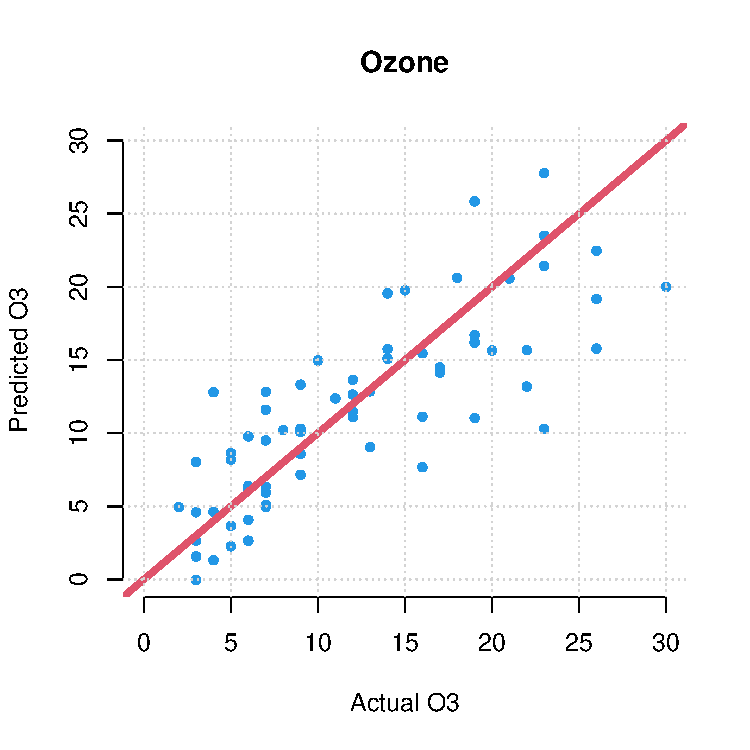
\includegraphics[width=.6\linewidth]{Figures/O3.pdf}
% \caption{Fitted QR model vs. observed values for $q=1/2$ for the ozone data.}\label{O3}
% \end{figure} 

%\clearpage
\bibliographystyle{abbrvnat}
\begin{thebibliography}{99}
\bibitem{SEMMS}
{\rm Bar, H.~Y., Booth, J.~G., {\rm and} Wells, M.~T.} (2020).
\newblock {A Scalable Empirical Bayes Approach to Variable Selection in
  Generalized Linear Models}.
\newblock \emph{Journal of Computational and Graphical Statistics}, {\bf  0}\penalty0 (0), \penalty0 1--12.
\end{thebibliography}
\end{document}
